\chapter{SAR images preprocessing}

\begin{figure}[H]
\centering
\includegraphics[width=0.8\columnwidth]{images/PHASE_mod1a.png}
\end{figure}

\section{Purpose and prerequisites}
The \textbf{Preprocessing} section prepares Sentinel-1 or COSMO-SkyMed scenes for StaMPS PSI. It handles image import or Sentinel-1 download, area-of-interest (AOI) definition, master selection, SNAP processing, interferogram formation, and StaMPS input export. It uses the shared PHASE installation; no project-local \texttt{.mlapp} or \texttt{snap2stamps} copy is required.

Install the PHASE release for your operating system and satisfy its checks for MATLAB, SNAP and the configured Python environment. Keep enough free storage for the SAR archives and substantially larger intermediate SNAP products. The first processing run may also need network access for orbit and elevation data. SNAP and external services are maintained independently of PHASE; if a download fails, inspect the \textbf{Run monitor} and the project logs before restarting.

\begin{quote}
\textcolor{orange}{\textbf{Scientific caution:}} The successful completion of a run means that the software finished, not that the interferograms are geodetically reliable. Inspect image overlap, orbit direction, burst coverage, coherence, phase quality, and the final AOI before proceeding to PSI.
\end{quote}

\section{Start a project}
Launch \textbf{PHASE}. Choose \textbf{New project} to create a workspace in any writable location, or \textbf{Open project} to resume one. The hub shows the project name, counts of input files, StaMPS datasets and exports, and the suggested next stage. Select \textbf{Preprocessing} from the hub navigation; the four section buttons remain available while working in a module. A green stage indicator is based on detected outputs and is not a data-quality assessment.

New projects separate input data, internal processing, final results and logs into four numbered top-level folders, as listed in the Introduction. PHASE creates the needed subdirectories. Do not rename or edit active processing directories, especially when resuming a stack. Older projects may retain their original layout.

\section{Images and AOI}
\subsection{Sentinel-1 download or import}
Use the module's \textbf{Download} section to search for and download Sentinel-1 scenes through the ASF service, or use \textbf{Import images} to add local archives. An ASF account and valid access may be required by the service. For a coherent stack, use compatible acquisition geometry, orbit direction, polarization, mode, and overlapping coverage. The map helps delimit the search and inspect the scene footprints; the later AOI controls what PHASE processes.

\begin{figure}[htbp]
\centering
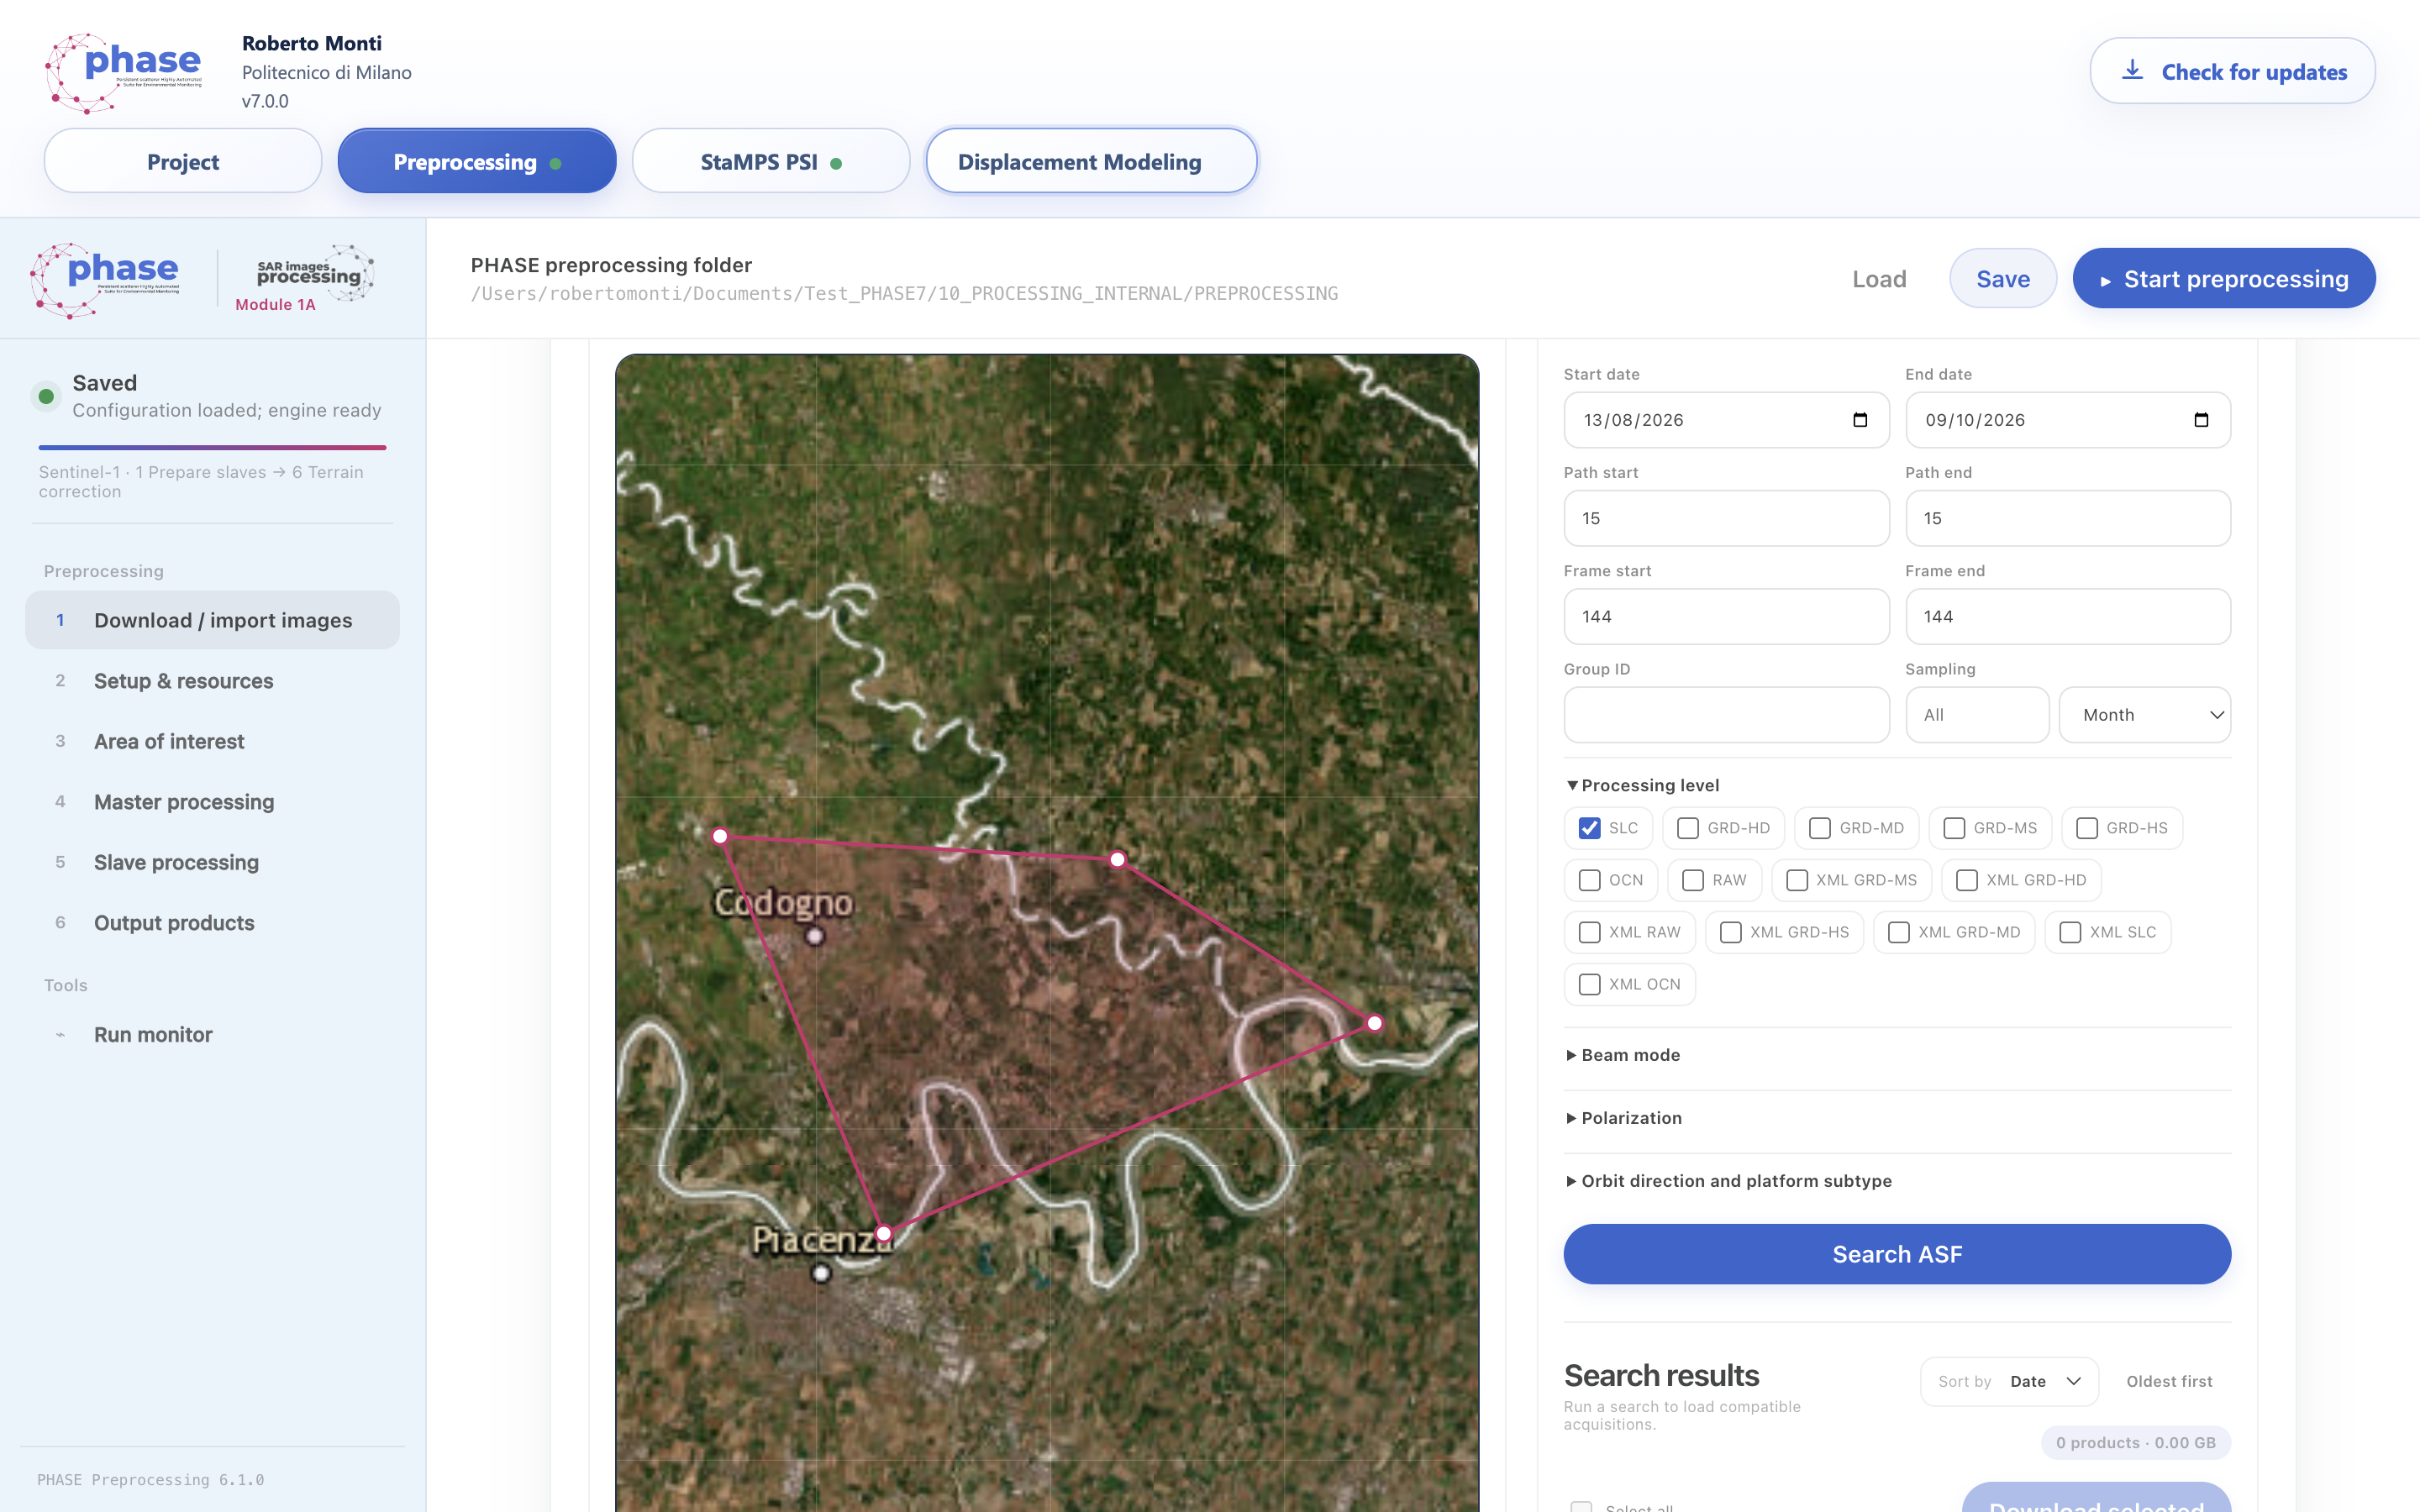
\includegraphics[width=\textwidth]{images/Screenshot 2026-10-11 alle 23.10.22.png}
\caption{Sentinel-1 search in the integrated Preprocessing section. The map and ASF filters are shown together; the displayed search parameters are examples, not recommended settings for every project.}
\label{fig:phase7-asf}
\end{figure}

For an existing Sentinel-1 stack, the \textbf{Update stack} workflow searches for and processes newly available compatible images while retaining existing products. Review its options and back up valuable results before a substantial reprocessing operation. Importing images from a different project is possible, but first confirm that they truly belong to the same geometry and acquisition series.

\subsection{COSMO-SkyMed scenes}
COSMO-SkyMed (CSK/CSG) scenes are obtained through the applicable data provider and imported locally. Check that the product type is supported by the selected preprocessing workflow and that the scenes share acquisition geometry and adequate AOI overlap. Access conditions, file formats, and mission-specific restrictions are controlled by the provider; consult its current documentation. PHASE does not convert an incompatible set of acquisitions into a valid interferometric stack.

\subsection{AOI selection}
Open the \textbf{Area of Interest} panel and draw the processing box on the map over the displayed footprint. Keep a margin around the target area so that registration and later quality checks have usable coverage. The selected geographic bounds are transferred to the processing parameters. A satellite basemap requires network access; if tiles are unavailable, verify the numerical bounds and footprint rather than assuming that a blank basemap means missing SAR coverage.

\begin{figure}[htbp]
\centering
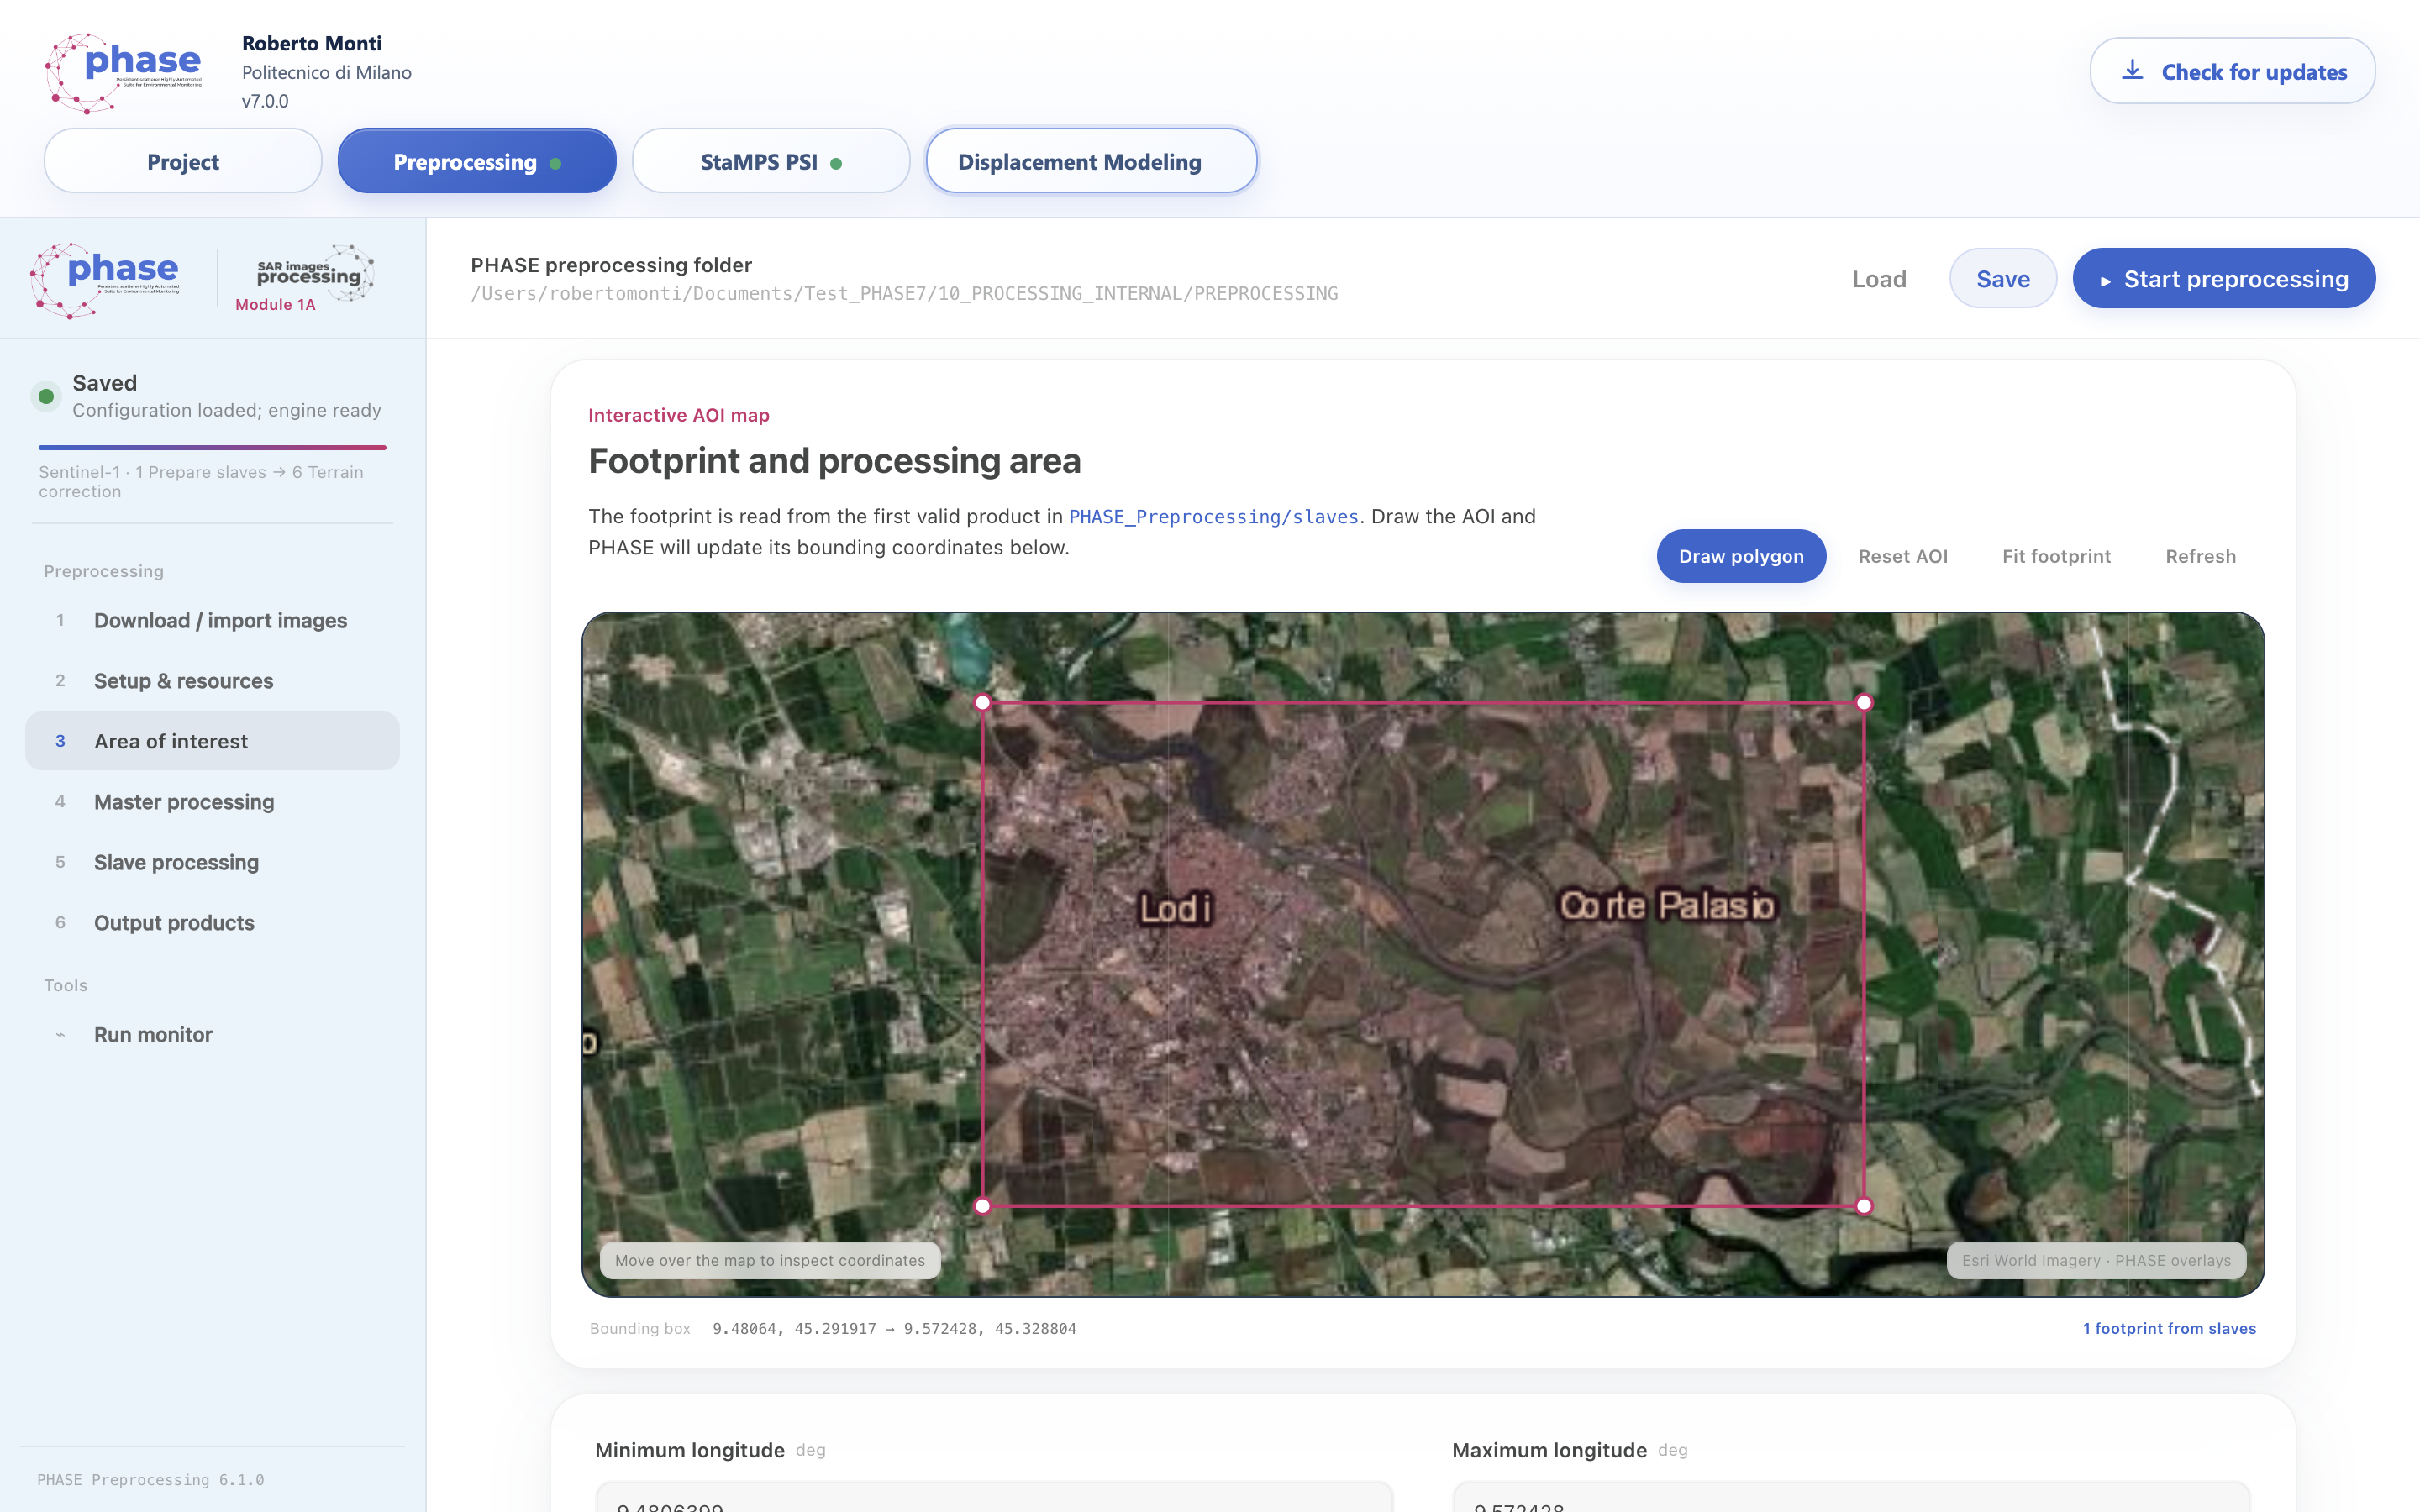
\includegraphics[width=\textwidth]{images/Screenshot 2026-10-11 alle 23.10.41.png}
\caption{Interactive processing AOI in PHASE 7. The pink polygon and numerical bounds illustrate the area selected for this example project.}
\label{fig:phase7-aoi}
\end{figure}

\section{Master selection and parameters}
PHASE can propose a master based on the available stack. Review its position in time and spatial overlap. For manual selection, use the date picker: it is constrained to acquisition dates found in the imported slaves and writes the date in the format required by the processing engine. Do not type an arbitrary date that is absent from the stack. For Sentinel-1, PHASE derives the needed swath/burst choices from scene metadata and AOI; verify them when the footprint is marginal or crosses burst boundaries.

In the \textbf{Master processing}, \textbf{Slaves processing}, \textbf{Coherence and LIA}, and \textbf{Computational resources} sections, review the active controls before launching a run. SNAP's \texttt{gpt} location, memory, concurrency, temporary storage and DEM choice affect performance and reproducibility. PHASE applies platform-aware limits where available, but an unusually large AOI or stack can still exceed system resources. Reduce AOI or concurrency if repeated runs exhaust memory. Use an external DEM only after checking its reference system, NoData value and full spatial coverage (see Appendix A).

\section{Run and interpret progress}
Save the configuration, then choose \textbf{Start preprocessing}. The \textbf{Run monitor} shows the current operation, elapsed time, a progress estimate, the slave being handled and a live log. Major operations include split/orbit handling, coregistration, interferogram and topographic-phase processing, StaMPS export, average intensity, and optional coherence/local-incidence-angle outputs. A percentage is an estimate of completed operations, not a time-to-finish prediction; an individual SNAP operation may take much longer than its neighbors.

If a run fails, preserve its error log and identify the exact scene and operation before retrying. When resuming from a slave step, PHASE can reuse existing master products; do not remove those products manually unless the run monitor explicitly instructs you to start from scratch. When preprocessing finishes, return to the hub or open \textbf{StaMPS PSI} through the persistent navigation. PHASE does not launch a separate StaMPS app. Check the expected StaMPS dataset and interferogram count before starting PSI.

\section{Processing outline}
For Sentinel-1, the principal SNAP operations include TOPSAR splitting and orbit application, back-geocoding and optional enhanced spectral diversity, interferogram formation, debursting, topographic-phase removal, StaMPS export, and terrain-corrected auxiliary layers. COSMO-SkyMed follows its own subset, stack, registration, interferogram and export path. The order and optional operations depend on the selected configuration; the run log is the authoritative record for a specific project.

\section{Troubleshooting}
\begin{description}[style=nextline]
\item[Missing basemap] Verify internet access and tile-service availability. Continue only after independently checking AOI coordinates and footprint.
\item[Orbit or DEM download failure] Check external-service connectivity and SNAP logs. If appropriate, provide a verified external DEM. Avoid treating an incomplete orbit/DEM step as a successful run.
\item[SNAP memory or process failure] Reduce simultaneous workers, AOI or stack size and confirm adequate free disk space. Keep the error log so that a reproducible failure can be distinguished from transient resource pressure.
\item[No suitable master or burst overlap] Recheck scene geometry, orbit direction, selected AOI and acquisition dates; do not force a non-overlapping master.
\end{description}
